\documentclass[conference]{IEEEtran}
% Two-column IEEE conference format. For the two-sided journal layout use:
% \documentclass[journal,twoside]{IEEEtran}
\usepackage[T1]{fontenc}
\usepackage{graphicx}
\usepackage{amsmath,amssymb}
\usepackage{booktabs}
\usepackage{url}
\usepackage[hidelinks]{hyperref}
\graphicspath{{../../figures/paper/}}
\renewcommand{\dbltopfraction}{0.9}\renewcommand{\topfraction}{0.9}\renewcommand{\textfraction}{0.07}\renewcommand{\dblfloatpagefraction}{0.8}\setcounter{dbltopnumber}{2}
\newcommand{\unv}{\textsuperscript{\dag}}

\begin{document}

\title{Pavlov's Dog as an Evolved Learner: Ecological Statistics Determine When Conditioning Emerges and Why It Ignores Its Consequences}

\author{\IEEEauthorblockN{Ronak Daniel}
\IEEEauthorblockA{\textit{Draft v0.1, 19 November 2026 --- not for circulation}}}

\maketitle

\begin{abstract}
Pavlov's dogs salivated to a bell that predicted food, and later experiments showed that the response persists even when salivating cancels the food. We asked whether such a conditioned response emerges on its own in artificial agents whose only action is salivation and whose only objective is physiological: saliva improves digestion and costs energy. Recurrent agents were evolved with evolution strategies over simulated lifetimes in which the cue that predicted food changed from lifetime to lifetime. Nothing in the objective referred to cues, and the laboratory tests were never part of evolution. Frozen and placed in a simulated Pavlov laboratory with a bell they had never encountered, agents from 20 pre-registered evolutionary runs acquired a conditioned-response-like (CR-like) salivation to the bell within a few pairings (bell$-$metronome discrimination 0.60, 95\% CI [0.53, 0.67]; none before pairing). The response depended on the bell--food contingency, partly extinguished, and was insensitive to an omission contingency (omission sensitivity index 0.01 [0.00, 0.02]): agents kept salivating although this cost them 84\% of the food. Sister lineages evolved under different response--outcome statistics showed that ecology decides whether a CR exists, not whether it is Pavlovian. Exploratory experiments indicate that inborn responses evolve to cues of fixed meaning and conditioning to cues of variable meaning, that the association is stored in a few cue-specific recurrent units, and that the evolved learner, unlike Rescorla--Wagner and temporal-difference models, shows no blocking.
\end{abstract}

\begin{IEEEkeywords}
classical conditioning, meta-reinforcement learning, evolution strategies, Pavlovian control, omission, recurrent neural networks
\end{IEEEkeywords}

\section{Introduction}
Classical conditioning is usually modelled in two parts. Prediction models such as Rescorla--Wagner (RW) \cite{rw72} and temporal-difference (TD) learning \cite{sb90} explain how a conditioned stimulus (CS) comes to predict an unconditioned stimulus (US). Agent models of Pavlovian control then attach a fixed response to that prediction by construction \cite{modayil14,butcher22}. Both take the link between prediction and response as given. A functional view \cite{domjan05,hollis97} instead holds that conditioned responses exist because they improve how an animal deals with the US: saliva secreted before food arrives speeds digestion. On this view the prediction--response link is itself a product of evolution, and so is its most puzzling property. In omission experiments \cite{sheffield65,williams69}, animals keep producing the CR even when it cancels the US. Normative accounts explain this as a hard-wired, outcome-insensitive controller that is usually right \cite{dayan06}.

Theory of the evolution of learning predicts when learning should be favoured over fixed behaviour: when the world varies between generations but is predictable within a lifetime \cite{stephens91,katsnelson12}. Meta-reinforcement learning (meta-RL) makes this testable: an outer optimisation loop over many lifetimes produces a recurrent network whose fixed weights implement a within-lifetime learning algorithm in its activations \cite{wang18,binz23}. Meta-learned agents have been compared with RW-type models in decision tasks \cite{schubert24}, but to our knowledge none has been taken through Pavlov's protocols or an omission test.

We built such a test. The agent's only effector is salivation, and its only consequence is physiological. An outer loop (evolution strategies, the analogue of evolution) optimises digestion over many lifetimes in an ecology where the meaning of cues varies between lifetimes. The inner loop is a single lifetime with frozen weights, in which any learning must happen in recurrent activity. Evolved agents are then frozen and run, blind, through a simulated laboratory that evolution never saw. We ask whether a CR-like response to a novel bell emerges (Q1); whether it is Pavlovian or instrumental, and what decides this (Q2); which classical phenomena emerge (Q3); and how it is implemented (Q4). Q1 and Q2 were tested in a pre-registered confirmatory study with 20 independent evolutionary histories; the rest is exploratory.

\textit{Spontaneity.} We call the CR spontaneous because (i) reward is physiology only and never references cues, trials or the lab; (ii) salivation affects only the saliva level; (iii) which channel predicts food is resampled every lifetime, so no channel---in particular not the lab's bell channel---has an innate meaning; (iv) there are no auxiliary losses; (v) weights are frozen in the lab; and (vi) the lab protocols and the omission contingency never occur during evolution. These invariants are enforced by automated tests. What we build in, and state openly, is the premise that saliva improves digestion, and standard meta-RL inputs (food in the mouth, own saliva level, previous action and reward).

\section{Methods}

\subsection{Physiology and reward}
Saliva $S_t\in[0,1)$ evolves as
\begin{equation}
S_{t+1}=S_t+k_{\uparrow}\,u_t\,(1-S_t)-k_{\downarrow}\,S_t,
\end{equation}
with $k_{\uparrow}=0.35$, $k_{\downarrow}=0.15$ and sampled action $u_t\in\{0,1\}$. A food item stays in the mouth for $D=3$ ticks and yields, per tick,
\begin{equation}
e_t=\tfrac{E}{D}\,[\,b_0+(1-b_0)\,S_t\,],\qquad r_t=e_t-c\,u_t,
\end{equation}
with $E=1$, $b_0=0.3$ and $c=0.01$. These values were fixed by an oracle analysis of the physiology alone (anticipatory salivation must pay), never by laboratory metrics.

\subsection{Ecology}
A lifetime lasts 3000 ticks. There are four cue channels and one stimulus at a time; events start at a per-tick rate drawn per lifetime from $U(1/40,1/20)$. One predictive cue (two with probability 0.5) predicts food at an inter-stimulus interval (ISI) drawn from $\{3,\dots,12\}$ with contingency $P(\mathrm{US}\mid\mathrm{CS})\sim U(0.5,1)$; predictive and distractor channels share all temporal statistics. Cues are delay cues. With probability $q$ ($q=1$ in all confirmatory runs) the mapping from cue roles to channels is permuted for the lifetime. Predictive cues toggle between active and silent with hazard $1/1500$ and revert to their original contingency with probability 0.5; unsignalled food occurs at up to 0.005 per tick. Sister arms add, in a fraction $v=0.5$ of lifetimes, either impaired digestion (efficiency $b_0(1-S_t)$, equal to the normal efficiency at $S=0$) or a partial-omission gate (salivating during a predictive cue's window halves that trial's US probability).

\subsection{Agent and outer loop}
The agent is a gated recurrent unit (GRU, 64 units) over a 64-unit $\tanh$ embedding of [cues, food in mouth, $S_t$, $u_{t-1}$, $r_{t-1}$], with a Bernoulli salivation head (probability $p_t$) and a value head unused by the outer loop. There are no auxiliary losses. Weights were optimised with OpenAI evolution strategies \cite{salimans17}: antithetic sampling, centred-rank fitness shaping, population 64, 8 lifetimes per member, $\sigma=0.03$, Adam with learning rate 0.02 and weight decay 0.005. Ancestors evolved for 4000 generations from scratch; sisters for 2000 generations from their ancestor's final weights with a fresh optimiser state. Training resumed exactly from checkpoints after interruptions.

\subsection{Laboratory}
Agents were frozen (no optimiser is reachable from the lab code). Each protocol ran 32 subjects from a zero hidden state with schedules fixed by a lab seed, identical for every agent. Bell (CS+) and metronome (CS$-$) occupied two random channels per subject; CS duration 6 ticks plus the US tick; inter-trial intervals $U\{15,\dots,35\}$. Every protocol began with 4 CS+ and 4 CS$-$ trials without food. Protocols: standard (25 paired CS+, 25 CS$-$, 20 extinction trials, 300 empty ticks, 5 recovery trials); truly random; CS alone; US alone; omission (40 CS+ trials whose food is cancelled if the agent salivates during the CS, plus 20 CS$-$) with a yoked partner receiving identical cues and food; and positive contingency with a yoked partner. The CR on a trial is
\begin{equation}
\mathrm{CR}=\overline{p}_{[\,t_{\mathrm{US}}-3,\,t_{\mathrm{US}})}-\overline{p}_{[\,t_{\mathrm{CS}}-10,\,t_{\mathrm{CS}})},
\end{equation}
and the omission sensitivity index is
\begin{equation}
\mathrm{OSI}=\mathrm{clip}\!\left(1-\mathrm{CR}_{\mathrm{omission}}/\mathrm{CR}_{\mathrm{yoked}},\,0,\,1\right),
\end{equation}
computed on the last 15 CS+ trials and undefined when $\mathrm{CR}_{\mathrm{yoked}}<0.05$. The scheduler cannot read agent outputs; the only route from behaviour to the schedule is the declared contingency.

\subsection{Pre-registration and statistics}
Pilot studies used seeds 100--199. Confirmatory seeds (0--99) were locked until the pre-registration was frozen (git tag \texttt{prereg-v1}). Each ancestor $a\in\{0,\dots,19\}$ was split into a stable, a digestion-variable and a partial-omission sister. The unit of analysis is the evolutionary seed ($N=20$); lab measures are means over 32 subjects. The 11 confirmatory tests form one Holm--Bonferroni family ($\alpha=0.05$); two-tailed tests count only in the predicted direction; bounds and equivalence use one-sided $t$-tests and TOST. Effect sizes are means with 95\% percentile bootstrap CIs (10\,000 resamples) and Cohen's $d_z$. No seed was excluded. Disclosed deviations from the draft pre-registration, all made before any confirmatory run: the original hypothesis H2 (response--outcome variability yields omission sensitivity) failed in every pilot and was replaced by the pilot-derived H2$'$; trial windows were aligned with the implemented protocols; and the paired test window was matched to the controls' five unreinforced trials.

\section{Results}

\subsection{Agents acquire a CR-like response to a novel bell (H1)}
Evolved ancestors achieved a training return of 13.3, above a reflex that salivates only once food is in the mouth (11.6) and closing 57\% of the gap to the best cue-reading oracle (14.6); 17 of 20 met the pre-registered training criterion of 50\% (all 20 were analysed). In their training world they salivated with probability 0.43 before an expected US and 0.05 elsewhere.

Before any pairing, agents did not discriminate the bell from the metronome ($-0.004$ [$-0.015$, 0.008]). After pairing, the response to the bell rose to asymptote within about two trials while the response to the metronome did not (Fig.~\ref{fig:acq}). Discrimination over the last 10 acquisition trials was 0.60 [0.53, 0.67] (H1a, $d_z=3.9$) and its increase from the naive phase 0.60 [0.54, 0.67] (H1b). After truly-random exposure the bell's CR was 0.36 [0.31, 0.41] lower than after pairing (H1c), and after food alone 0.40 [0.35, 0.46] lower (H1d) (Fig.~\ref{fig:ctrl}).

\begin{figure*}[!t]
\centering
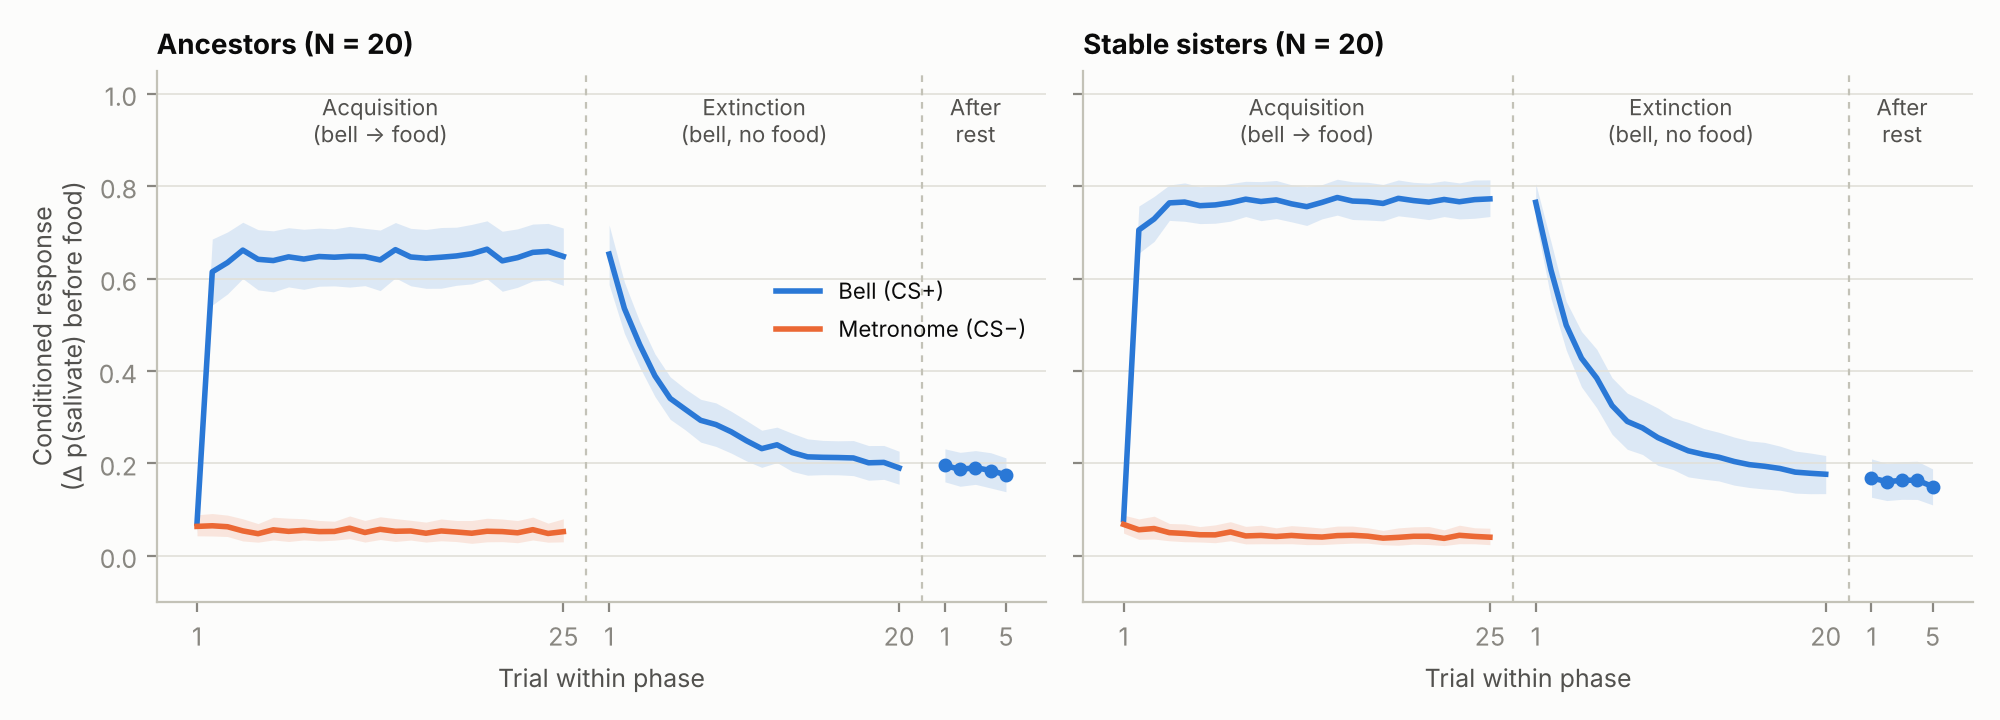
\includegraphics[width=\textwidth]{fig1_acquisition_extinction.png}
\caption{Acquisition, extinction and post-rest test in frozen ancestors (left) and stable sisters (right). Lines: mean CR over 20 seeds (each the mean of 32 lab subjects); bands: 95\% bootstrap CI.}
\label{fig:acq}
\end{figure*}

\begin{figure*}[!t]
\centering
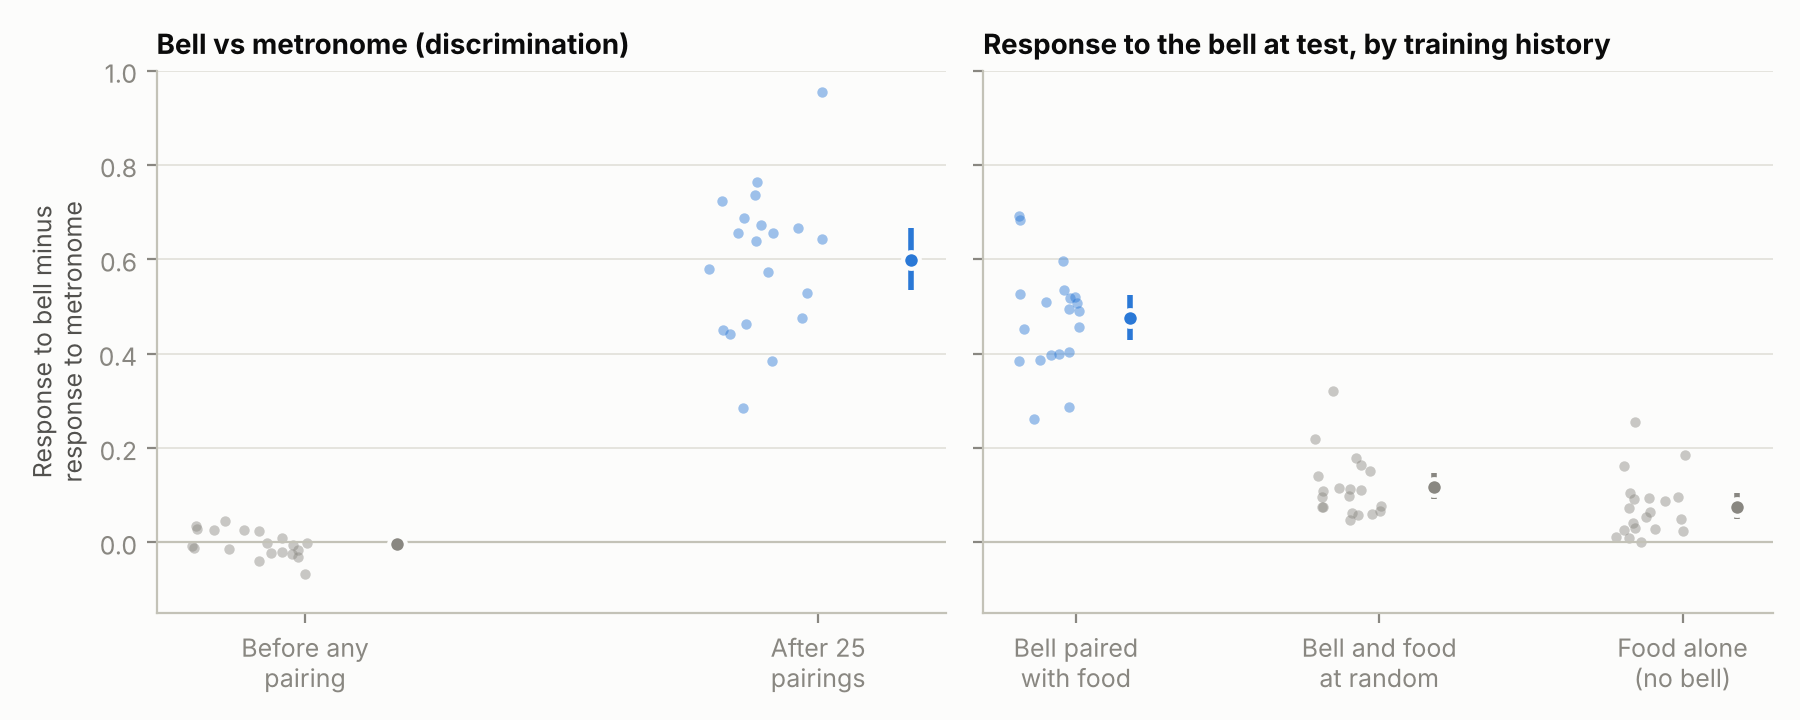
\includegraphics[width=0.85\textwidth]{fig2_controls.png}
\caption{Discrimination before vs after pairing (left) and the bell's CR at test after pairing, truly-random exposure or food alone (right). Dots: seeds; large marker: mean with 95\% CI.}
\label{fig:ctrl}
\end{figure*}

\subsection{The CR extinguishes and ignores its consequences (H3)}
Without food, the CR declined to 0.20 over 20 trials, about a third of its acquisition level (0.5$\cdot$acquisition $-$ extinction $=0.12$ [0.08, 0.16], H3a); extinction was partial. Under omission, agents salivated as much as their yoked partners or slightly more (0.45 vs 0.41; Fig.~\ref{fig:om}) and received only 16\% of the available food. OSI was 0.010 [0.001, 0.023], below the pre-registered margin of 0.2 (H3b). A positive contingency had no effect ($-0.003$ [$-0.009$, 0.002], equivalent to zero within $\pm0.1$, H3c). The evolved CR is therefore Pavlovian-like: it follows the stimulus--outcome relation and ignores the response--outcome relation.

\begin{figure*}[!t]
\centering
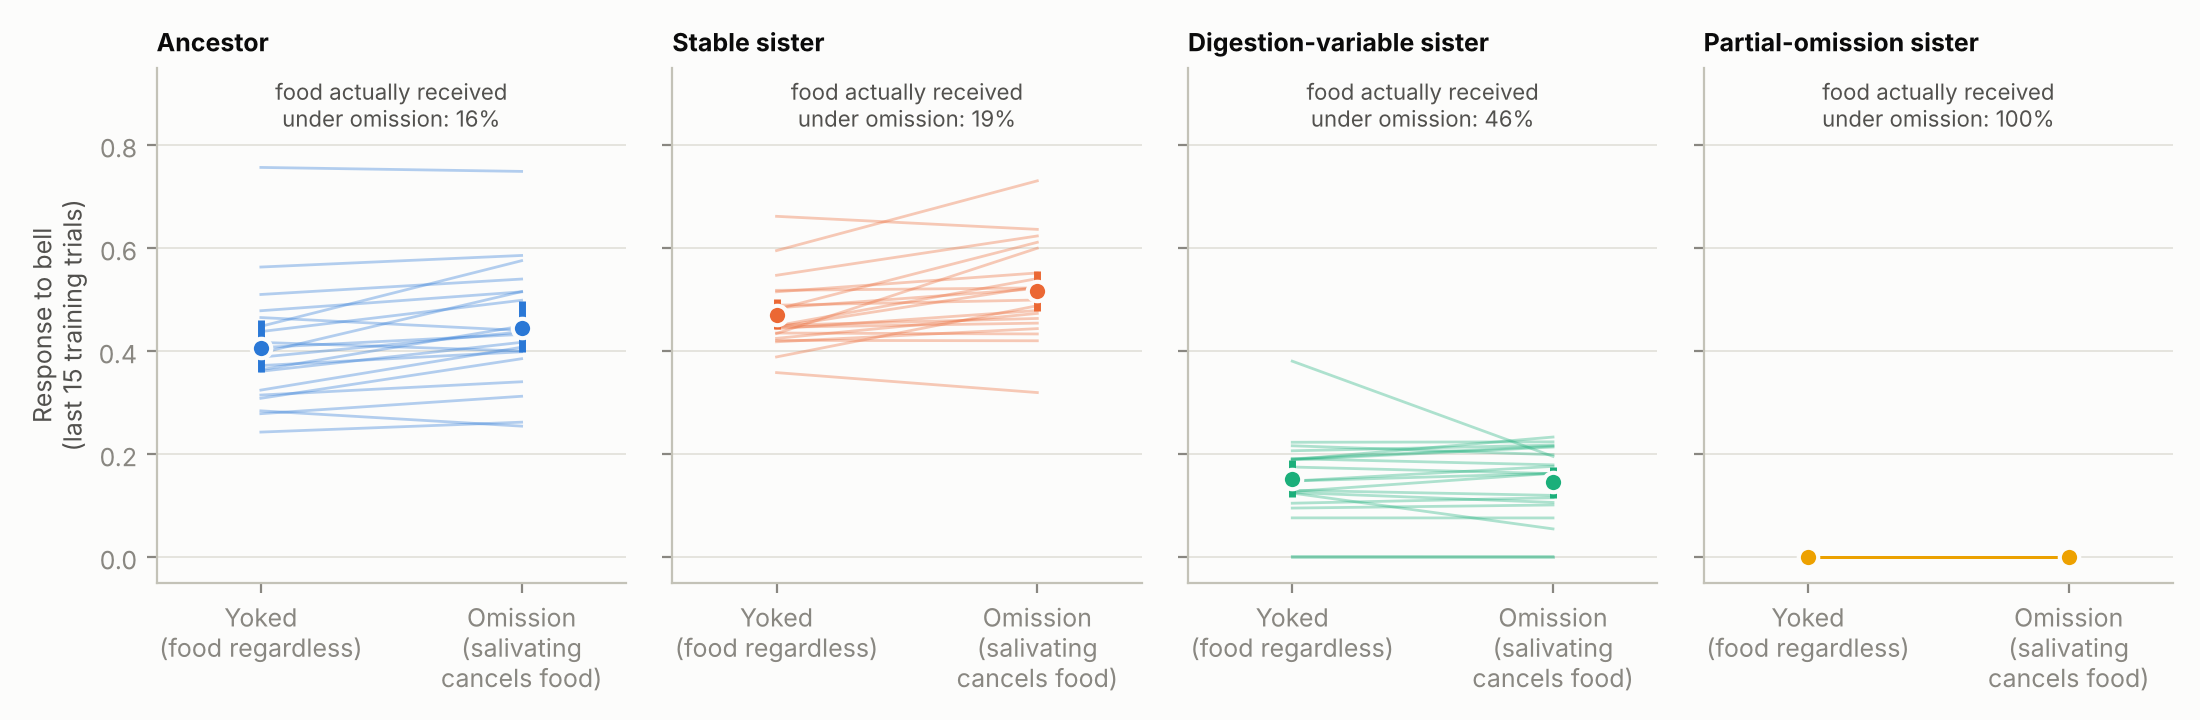
\includegraphics[width=\textwidth]{fig3_omission.png}
\caption{CR under omission vs the yoked partner, per arm. Lines: seeds. Text: fraction of the available food received under omission.}
\label{fig:om}
\end{figure*}

\subsection{Ecology decides whether a CR exists, not whether it is Pavlovian (H2$'$)}
Digestion-variable sisters evolved genuine within-lifetime response--outcome learning: their probability of salivating with food in the mouth differed by 0.65 between normal and impaired-digestion lifetimes, against $-0.03$ in their ancestors (difference 0.68 [0.58, 0.75], H2$'$b). Their bell CR was weaker (discrimination 0.10 vs 0.73 in stable sisters) but still omission-insensitive (OSI 0.08 [0.02, 0.17], $n=18$, H2$'$a). Partial-omission sisters abandoned the CR: acquired discrimination was 0.000 in all 20 lineages (difference from stable sisters $-0.73$ [$-0.77$, $-0.68$], H2$'$c; below 0.1, H2$'$d); these near-deterministic values are reported as magnitudes. Evolution never produced an omission-sensitive CR (Fig.~\ref{fig:arms}). All 11 pre-registered tests were supported.

\begin{figure*}[!t]
\centering
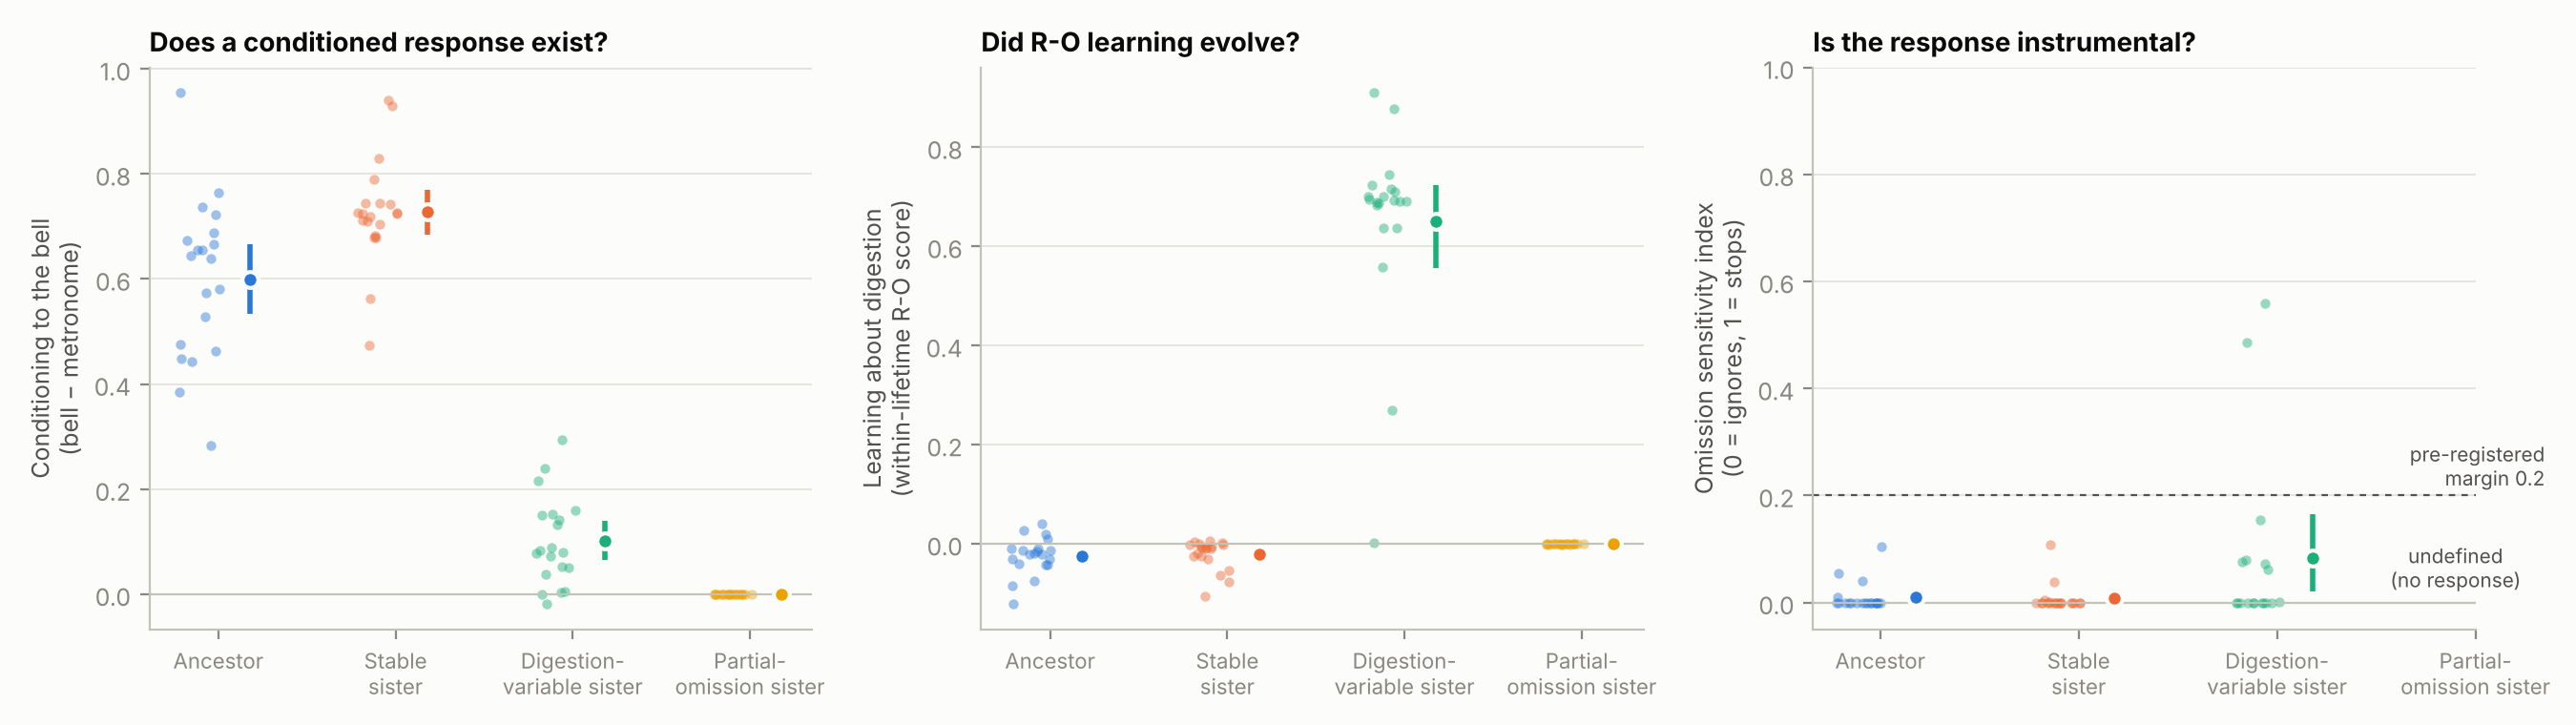
\includegraphics[width=\textwidth]{fig4_ecology_arms.png}
\caption{Per arm: conditioning strength, within-lifetime response--outcome learning, and OSI. Dots: seeds.}
\label{fig:arms}
\end{figure*}

\subsection{Fixed meanings yield inborn responses, variable meanings learning (exploratory)}
We evolved five ancestors with fixed cue meanings ($q=0$) and five with half the lifetimes reshuffled ($q=0.5$). At $q=0$, agents salivated to the always-predictive channel on first encounter (naive CR 0.85 [0.76, 0.92] vs 0.11 at $q=1$). A pre-stated prediction of no learning on the other channels partly failed (0.37); a post-hoc split by channel (Fig.~\ref{fig:svar}) showed that agents learned channel 1, which is predictive in half of all lifetimes (0.80), and ignored channels 2--3, which never predict food at $q=0$ ($-0.05$). The same held at $q=0.5$, although channels 2--3 predict food in about one lifetime in five there; only at $q=1$ were all channels learned. The pattern resembles selective associability and needs a dedicated test.

\begin{figure*}[!t]
\centering
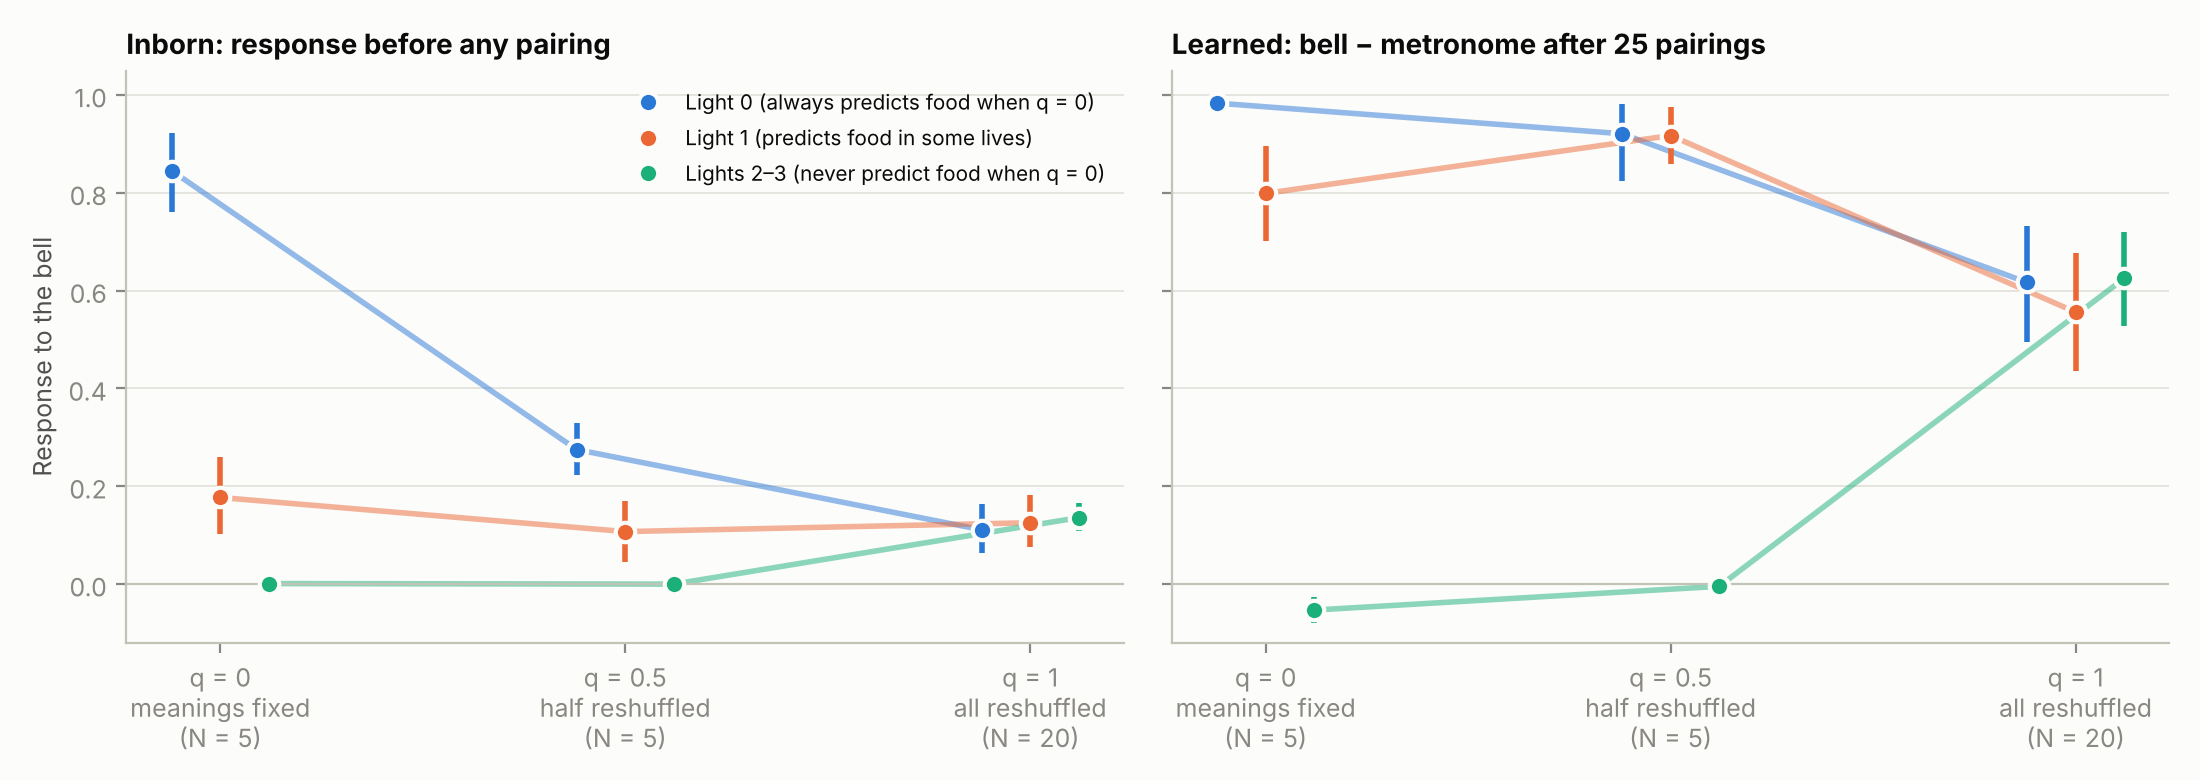
\includegraphics[width=0.85\textwidth]{fig5_so_variability.png}
\caption{Naive (left) and acquired (right) response by bell channel and cue-meaning variability $q$ (exploratory; channel split post hoc).}
\label{fig:svar}
\end{figure*}

\subsection{The association lives in a few cue-specific units (exploratory)}
A linear probe decoded an expectation of food from the recurrent state (held-out $R^2=0.59$ [0.54, 0.64]), but steering along the probe direction changed salivation no more than a random direction, so it is not the causal variable. Activation patching was informative: transplanting the 8 most-changed of 64 units from a trained state into the same subject's naive trial transferred 76\% [61, 90] of the acquired CR, and 16 units transferred all of it. A state from another subject trained on the same channel transferred equally well (81\%), whereas one trained on a different channel transferred nothing and reduced responding ($-26$\% [$-40$, $-12$]). The association is compact and indexed by input channel.

\subsection{A fast, non-competitive learner (exploratory)}
Table~\ref{tab:score} and Fig.~\ref{fig:ph} compare agents with RW, TD with a complete serial compound, and an instrumental Q-learner trained within the session (parameters fixed a priori). No post-Pavlovian phenomenon was clearly present in the ancestors. The added cue of a compound gained as much CR after its partner had been trained as in an overshadowing control (blocking $-0.005$), whereas RW and TD showed strong blocking. Pre-exposure did not slow acquisition, which reached asymptote after one pairing. Extinction after 50\% reinforcement was not slower once terminal levels are considered; responding did not rise across a 24-tick CS (it rose slightly across a 12-tick CS); second-order conditioning was tiny; and there was no spontaneous recovery. The instrumental learner never acquired an anticipatory response within a session.

\begin{table}[t]
\centering
\caption{Agents (20 ancestors, mean [95\% CI]) vs baseline learners}
\label{tab:score}
\footnotesize
\setlength{\tabcolsep}{3pt}
\begin{tabular}{@{}lccccc@{}}
\toprule
Measure & Anim. & Agents & RW & TD & Q \\
\midrule
Acquired discrim. & $>0$ & 0.60 [0.53, 0.67] & 1.00 & 0.55 & $-0.01$ \\
Paired $-$ random & $>0$ & 0.36 [0.31, 0.41] & 0.48 & 0.59 & $-0.03$ \\
Extinction ratio & $<1$ & 0.33 [0.26, 0.42] & 0.00 & 0.60 & --- \\
Spont.\ recovery & $>0$ & $-0.01$ [$-0.02$, 0.00] & 0.00 & $-0.05$ & 0.00 \\
OSI & $\approx0$ & 0.01 [0.00, 0.02] & 0 & 0 & n/a \\
Blocking & $<0$ & $-0.01$ [$-0.03$, 0.02] & $-0.28$ & $-0.16$ & 0 \\
Latent inhib. & $<0$ & $-0.02$ [$-0.04$, 0.01] & 0 & 0 & 0 \\
Inhib.\ of delay & $>0$ & 0.00 [0.00, 0.00] & 0 & 0.02 & 0 \\
Second-order & $>0$ & 0.01 [0.00, 0.03] & 0 & 0.01 & 0 \\
\bottomrule
\end{tabular}
\end{table}

\begin{figure*}[!t]
\centering
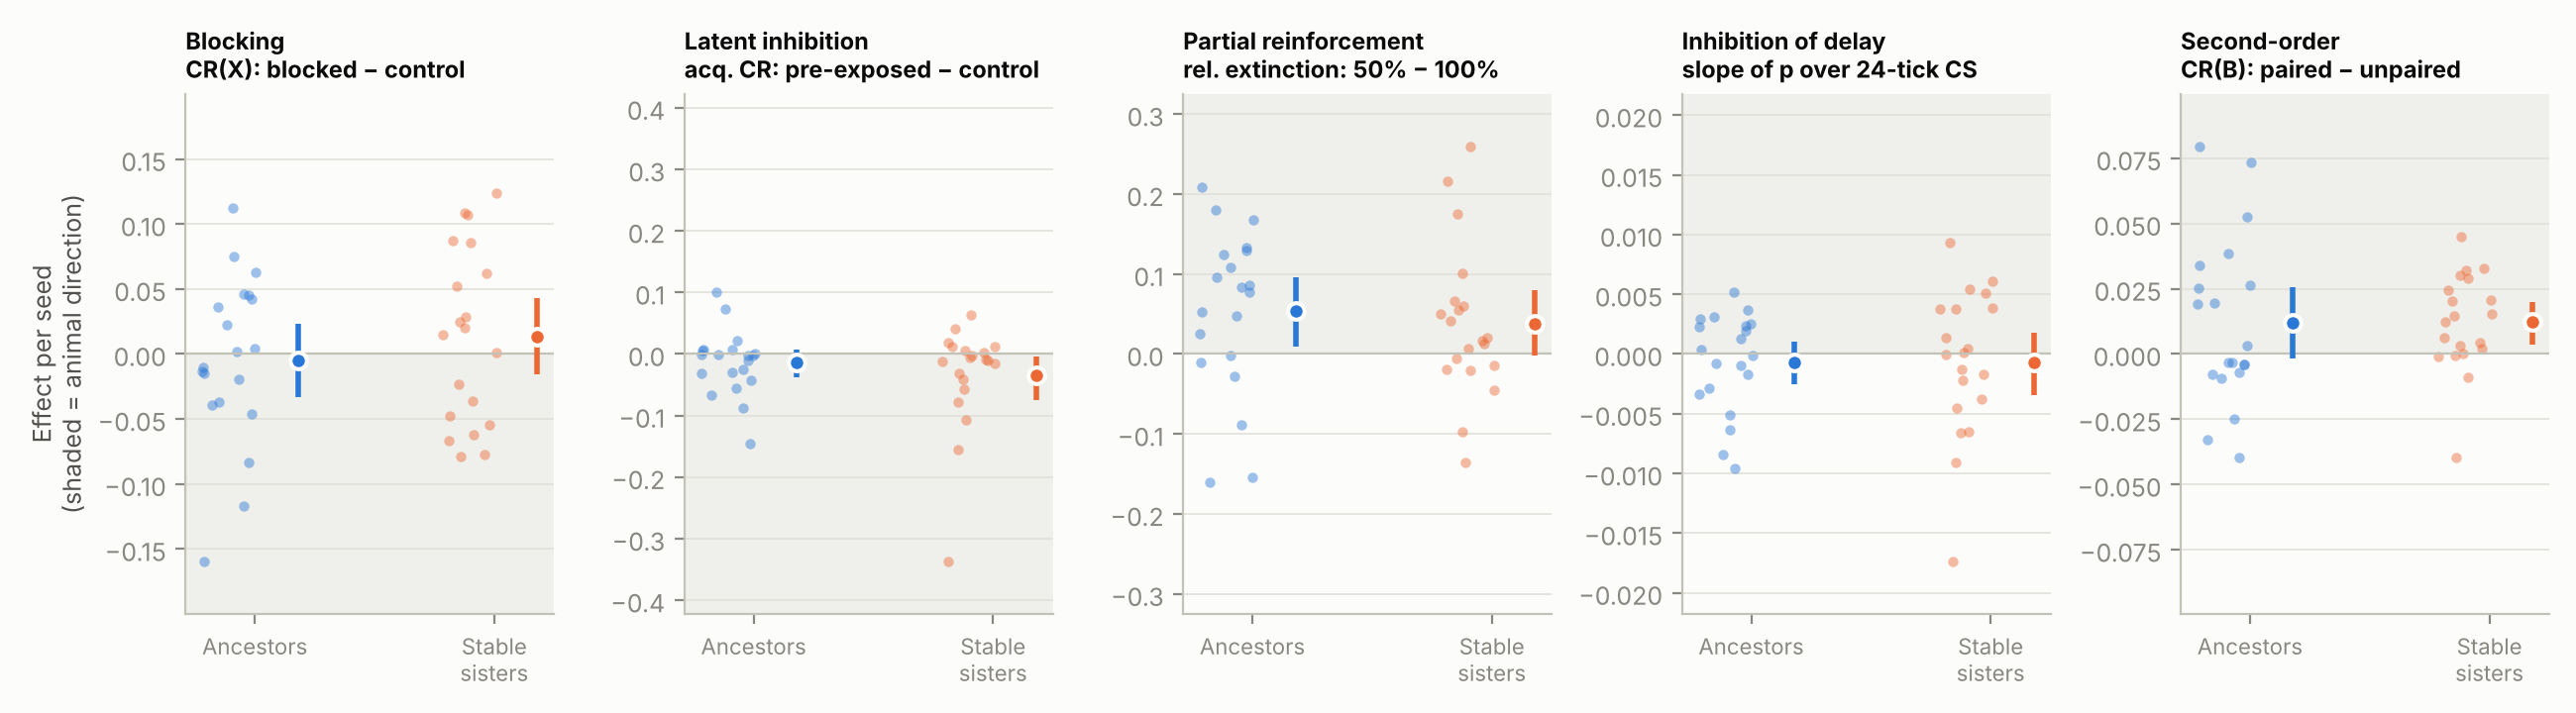
\includegraphics[width=\textwidth]{fig6_phenomena.png}
\caption{Phenomena battery. Per-seed effects in ancestors and stable sisters; the shaded half is the direction animals show.}
\label{fig:ph}
\end{figure*}

\section{Discussion}
Optimising nothing but digestion, over lifetimes in which cue meanings varied, produced agents that reproduce the core of Pavlov's findings in a laboratory they had never seen: a response to a novel bell that is acquired within a few pairings, depends on the bell--food contingency, extinguishes partly and persists when it costs the food.

\textit{Why outcome-insensitivity?} In the ancestors' world, salivating never changed whether food came, only how well it was digested; a response that follows the food prediction and ignores its own consequences is then optimal. The sister lineages sharpen this: given response--outcome variability, evolution either added separate learning about digestion while keeping the bell response Pavlovian, or removed the bell response, rather than bringing it under instrumental control, although an instrumental policy would have paid more. A four-times larger search (pilot) did not change this, but a stronger search might. The result supports the view of Pavlovian control as a cheap, usually adequate default \cite{dayan06}.

\textit{When does learning evolve?} Fixed meanings produced an inborn response and variable meanings produced learning, as theory predicts \cite{stephens91}; rarely relevant cues were neglected without any built-in attention mechanism.

\textit{What kind of learner?} The evolved learner is fast and channel-specific, with a compact memory of 8--16 units. It is not error-correcting in the RW sense: it shows no blocking, latent inhibition or partial-reinforcement extinction effect. We read these as boundary conditions set by the ecology, which presented one stimulus at a time and rarely changed contingencies within a life; evolving agents with compound cues is the direct test.

\textit{Limitations.} The ecology is simple; we tested two response--outcome families; several lab conditions are out of distribution (compounds, long CSs, long rests); exploratory results use fewer seeds or post-hoc splits; baseline parameters were not fitted; and we claim CR-like behaviour, not equivalence with animals.

\section{Conclusion}
A physiology-only objective in a world of shifting cue meanings is sufficient for a Pavlovian-like conditioned response, including its insensitivity to omission, to evolve without being built in. Ecology decided whether such a response exists; in no case did it become instrumental.

\section*{Data and code availability}
All code, configurations, logs, lab outputs, final checkpoints and the decision log are in the project repository; figures are regenerated from the results by a single script.

\begin{thebibliography}{99}
\footnotesize
\bibitem{rw72} R.~A. Rescorla and A.~R. Wagner, ``A theory of Pavlovian conditioning,'' 1972.\unv
\bibitem{sb90} R.~S. Sutton and A.~G. Barto, ``Time-derivative models of Pavlovian reinforcement,'' 1990.\unv
\bibitem{modayil14} J.~Modayil and R.~S. Sutton, ``Prediction driven behavior: learning predictions that drive fixed responses,'' 2014.\unv
\bibitem{butcher22} J.~Butcher, P.~M. Pilarski \textit{et al.}, ``Frost Hollow: Pavlovian signalling,'' arXiv:2203.09498, 2022.
\bibitem{domjan05} M.~Domjan, ``Pavlovian conditioning: a functional perspective,'' \textit{Annu. Rev. Psychol.}, vol.~56, 2005.
\bibitem{hollis97} K.~L. Hollis, ``Contemporary research on Pavlovian conditioning: a `new' functional analysis,'' \textit{Am. Psychol.}, 1997.\unv
\bibitem{sheffield65} F.~D. Sheffield, ``Relation between classical conditioning and instrumental learning,'' 1965.\unv
\bibitem{williams69} D.~R. Williams and H.~Williams, ``Auto-maintenance in the pigeon,'' \textit{J. Exp. Anal. Behav.}, 1969.\unv
\bibitem{dayan06} P.~Dayan, Y.~Niv, B.~Seymour and N.~D. Daw, ``The misbehavior of value and the discipline of the will,'' \textit{Neural Netw.}, 2006.\unv
\bibitem{stephens91} D.~W. Stephens, ``Change, regularity, and value in the evolution of animal learning,'' \textit{Behav. Ecol.}, 1991.\unv
\bibitem{katsnelson12} E.~Katsnelson \textit{et al.}, \textit{Proc. R. Soc. B}, 2012.\unv
\bibitem{wang18} J.~X. Wang \textit{et al.}, ``Prefrontal cortex as a meta-reinforcement learning system,'' \textit{Nat. Neurosci.}, 2018.\unv
\bibitem{binz23} M.~Binz \textit{et al.}, ``Meta-learned models of cognition,'' \textit{Behav. Brain Sci.}, 2023.\unv
\bibitem{salimans17} T.~Salimans, J.~Ho, X.~Chen, S.~Sidor and I.~Sutskever, ``Evolution strategies as a scalable alternative to reinforcement learning,'' arXiv:1703.03864, 2017.\unv
\bibitem{schubert24} J.~A. Schubert, A.~K. Jagadish, M.~Binz and E.~Schulz, arXiv:2402.03969, 2024.
\end{thebibliography}
\noindent\footnotesize{\unv\,Not yet verified against the source.}

\end{document}
